% ======================================================================
\section{Numerical Experiments}\label{sec:numerics}
Protocol, implementations and test families are those of M1 (Sec.~\ref{M1-subsec:protocol},
Table~\ref{M1-tab:families}). Python reference timings are single-threaded medians after a warm-up
(5 runs for $n\le2^{16}$, 3 above), on an otherwise idle machine. The current repo solver is cross-checked
under Octave in Table~\ref{M1-tab:xval} of M1, which includes the weighted and Tikhonov wrappers:
they agree with the Python reference to $\le4.2\times10^{-14}$.

\subsection{Weighted minimum norm}\label{subsec:Wnum}
\textbf{W1 (accuracy).} Diagonal weights $L=\operatorname{diag}(10^{\alpha u_j})$, $u_j\sim U[-\frac12,\frac12]$, for
$\alpha=0,2,\dots,12$, i.e.\ up to 12 orders of magnitude between the smallest and largest weight.
Leaf-block weights $L_\tau=\operatorname{chol}(I+\beta K_\tau)$ with a Gaussian smoothing kernel $K_\tau$
(width 3), $\beta=1,10^2,10^4$. Families F2 ($1024\times2048$), F3 ($683\times2046$) and F4
($1016\times2048$). The reference is the dense backward-stable solution
$L^{-1}\,\mathrm{QR}\text{-}\min\text{-}\mathrm{norm}(HL^{-1},b)$. Figure~\ref{fig:W}: the error follows
$\kappa(HL^{-1})\,u$, the conditioning of the weighted problem. It is at or below that line for
$\kappa\gtrsim30$, over 9 decades ($\kappa$ up to $10^{10}$); for better-conditioned cases it sits at a floor
of $1$--$10\times10^{-15}$, up to a few times above $\kappa u$. The weighted norm of the computed solution
matches the reference to 10 digits or better in every case. The block weights give errors of
$1$--$10\times10^{-15}$.

\textbf{W2 (scale).} F2 with $\alpha=6$ and manufactured weighted solutions
$x_\star=L^{-1}(HL^{-1})^*z$ (exact for the HSS matrix), up to $n=2^{19}$: the error stays at
$2.7\times10^{-15}$ and the residual at $6.4\times10^{-16}$. The cost is that of an unweighted solve,
$0.9$--$1.13\times$ from $n=2^{12}$ to $2^{19}$ (0.50\,s against 0.49\,s at $n=2^{16}$), because forming
$HL^{-1}$ touches only the leaves.

\begin{figure}[t]
\centering
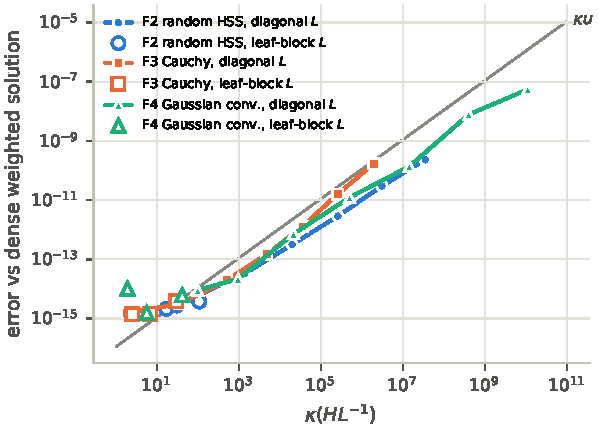
\includegraphics[width=0.55\textwidth]{figures/m2_weighted.pdf}
\caption{W1: weighted minimum-norm error against $\kappa(HL^{-1})$. Filled: diagonal $L$ with up to
12 decades of dynamic range. Open: leaf-block SPD $L$. Grey: $\kappa u$.}
\label{fig:W}
\end{figure}

\subsection{Tikhonov}\label{subsec:Tnum}
\textbf{T1 (accuracy along the $\lambda$ path).} $\lambda/\|H\|_2=10^{-8},\dots,10^{2}$ for wide
($1024\times2048$), square ($1536^2$) and tall ($2048\times1024$) F2, for the wide stride-2 ``valid''
Gaussian convolution ($1016\times2048$, F4) and for a square stride-1 ``same'' Gaussian convolution
($1536^2$). The reference is the dense SVD filter solution
$\sum_i\frac{\sigma_i}{\sigma_i^2+\lambda^2}(u_i^*b)v_i$. Figure~\ref{fig:T}a: errors of
$4\times10^{-15}$--$4\times10^{-13}$ for the F2 matrices and the wide convolution at every $\lambda$,
including the tall case, where plain min-norm does not apply. For the tall case $\kappa(H_a)u$ is a
loose bound: at $\lambda=10^{-8}\|H\|$ it is $10^{-8}$, the error $4\times10^{-13}$
(Sec.~\ref{sec:tikhonov}). For the square convolution ($\kappa=2.4\times10^7$) the error at small $\lambda$
is $5\times10^{-10}$, below $\kappa(H_a)u=2.6\times10^{-9}$, and it falls to $10^{-14}$ as $\lambda$ grows and
$\kappa(H_a)$ drops. At $\lambda=100\|H\|$ the relative error
of $x$ rises to $10^{-13}$: there $\|x\|\approx\|H\|\|s\|/\lambda$ is a small part of $z=(x,s)$. The general
form ($S$, $L$ diagonal with 2 decades each) matches a dense stacked least-squares solve to
$9\times10^{-13}$ ($\lambda=10^{-4}$) and $1.2\times10^{-14}$ ($\lambda=1$).

\textbf{T2/T3 (scale and cost).} Manufactured Tikhonov solutions ($x_\star=H^*z$,
$b=Hx_\star+\lambda^2z$, so $x_\lambda=x_\star$ exactly) with $\lambda=10^{-2}$: error
$1.5\times10^{-15}$ (wide, up to $n=2^{19}$) and $1.2\times10^{-15}$ (tall $m=2n$, up to $n=2^{18}$),
flat in $n$ (Figure~\ref{fig:T}c). The cost is linear (Figure~\ref{fig:T}b). A Tikhonov solve costs
$1.0$--$1.25\times$ a min-norm solve of the same wide $H$, up to $n=2^{19}$ (5.3\,s against 4.5\,s there).
That is below the factor $1+m/n=1.5$ one might expect from the wider leaves, because the size
reduction removes the extra columns at once (Sec.~\ref{sec:tikhonov}).

\begin{figure}[t]
\centering
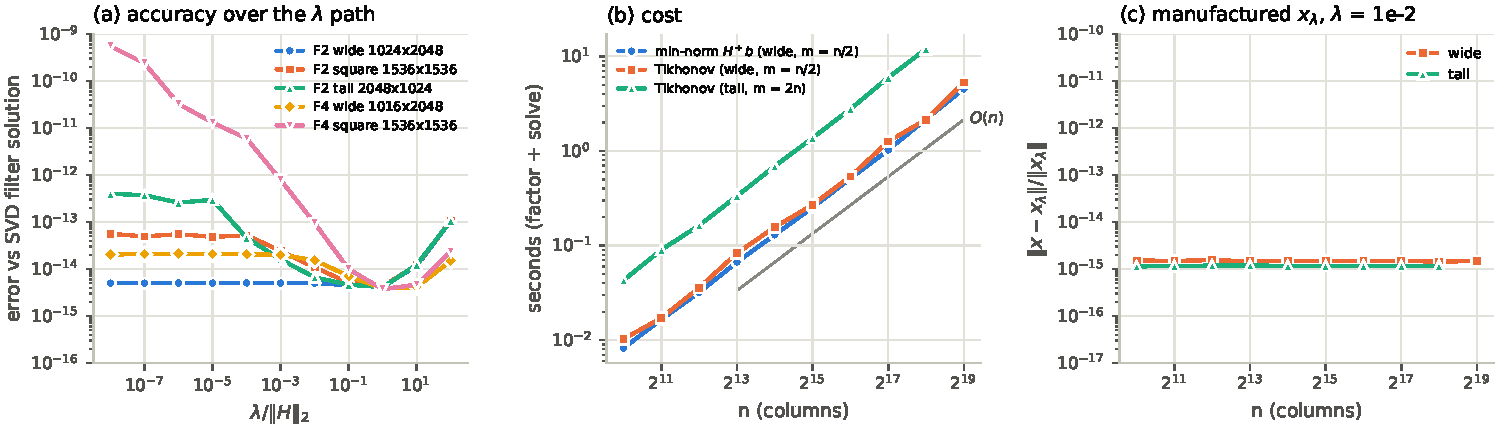
\includegraphics[width=\textwidth]{figures/m2_tikhonov.pdf}
\caption{T1--T3. (a) Error against the SVD filter solution along the $\lambda$ path. (b) Cost against
min-norm. (c) Manufactured Tikhonov solutions at scale.}
\label{fig:T}
\end{figure}

% ======================================================================
\section{Applications}\label{sec:apps}

\subsection{Basis pursuit: IRLS and Douglas--Rachford}\label{subsec:bp}
\emph{Problem.} Seismic reflectivity is modelled as a sparse spike train convolved with a band-pass
wavelet. $x_0\in\mathbb{R}^{4096}$ has 60 spikes (amplitudes $\pm[0.5,1.5]$, separation $\ge24$ samples).
$H$ is the Ricker wavelet ($\sigma=2.5$) convolution with stride 2, F4, $2038\times4096$, and
$b=Hx_0$. We solve basis pursuit, $\min\|x\|_1$ s.t.\ $Hx=b$, in two ways:
\begin{itemize}[leftmargin=1.4em,itemsep=1pt]
\item \textbf{IRLS} (Daubechies--DeVore--Fornasier--G\"unt\"urk~\cite{ddfg}). Repeat
$x^{k+1}=\operatorname*{arg\,min}_{Hx=b}\sum_jw_j^k|x_j|^2$ with $w_j^k=(|x_j^k|^2+\varepsilon_k^2)^{-1/2}$ and
$\varepsilon_{k+1}=\min(\varepsilon_k,|x^{k+1}|_{(s+1)}/n)$. \emph{The inner problem is exactly (W) with
$L=\operatorname{diag}(\sqrt{w^k})$.} The weights change every step, so each step is a fresh
factorization of $HL_k^{-1}$, and Theorem~\ref{thm:W} guarantees each inner solve is the exact
weighted minimum-norm point.
\item \textbf{Douglas--Rachford} on $\|x\|_1+\iota_{\{Hx=b\}}$:
$x^k=P(z^k)$, $z^{k+1}=z^k+\operatorname{soft}_\gamma(2x^k-z^k)-x^k$, $\gamma=0.05$, with the projection
$P(v)=v+H^+(b-Hv)$. Here $H$ never changes. It is factored \emph{once} and each step is one $O(nr)$
solve plus two HSS products. ADMM for the same problem has the same inner step.
\end{itemize}
\emph{Results} (Figure~\ref{fig:bp}). The minimum-norm solution has relative error 0.71: it is smooth,
not sparse. IRLS reaches $10^{-8}$ after 24 iterations and $1.6\times10^{-10}$ after about 33; DR reaches $8\times10^{-9}$ after 67.
One factorization costs 0.056\,s and one solve 0.0023\,s, so a DR step is $\approx24\times$ cheaper than
an IRLS step, and DR wins in wall time (0.25\,s against 1.5\,s to $10^{-8}$). The legacy MATLAB solver
refactors on every call, so with it DR loses that advantage. In the current code $H$ keeps its factors,
so the projection \texttt{v + H\textbackslash(b - H*v)} factors only on the first call.

\begin{figure}[t]
\centering
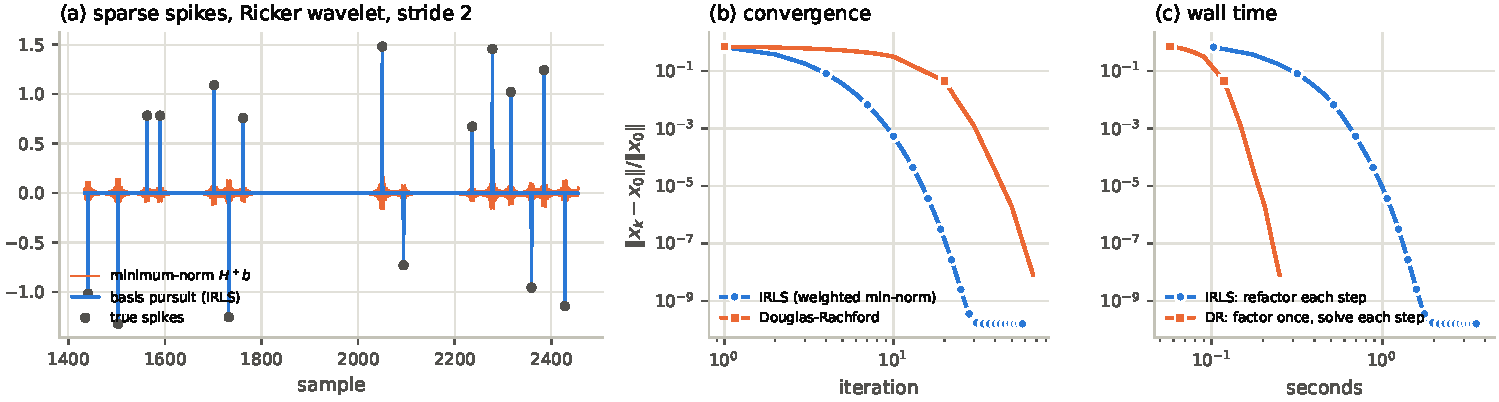
\includegraphics[width=\textwidth]{figures/m2_bp.pdf}
\caption{Basis pursuit for sparse-spike deconvolution. (a) Detail of the recovered spike train.
(b, c) Convergence in iterations and in wall time.}
\label{fig:bp}
\end{figure}

\subsection{Tikhonov deblurring and the choice of $\lambda$}\label{subsec:db}
The signal of M1, Sec.~\ref{M1-subsec:a2} ($n=4096$), Gaussian blur $\sigma=3$, stride 2, 1\% white noise.
The minimum-norm solution has error 94: it inverts the noise. A sweep of 23 values of $\lambda$ costs
0.07\,s per $\lambda$ (one factorization each). The discrepancy principle (largest $\lambda$ with
$\|Hx_\lambda-b\|\le1.01\|e\|$) gives $\lambda=0.32$ with error 0.046, against the best on the grid,
0.036 at $\lambda=0.56$ (Figure~\ref{fig:db}). The L-curve corner (maximum curvature) is at
$\lambda=0.032$, ten times smaller, with error 0.30: here the L-curve under-regularizes, a known
limitation for smooth solutions~\cite{hanke}. The discrepancy principle needs $\|e\|$, which this test
knows.

\begin{figure}[t]
\centering
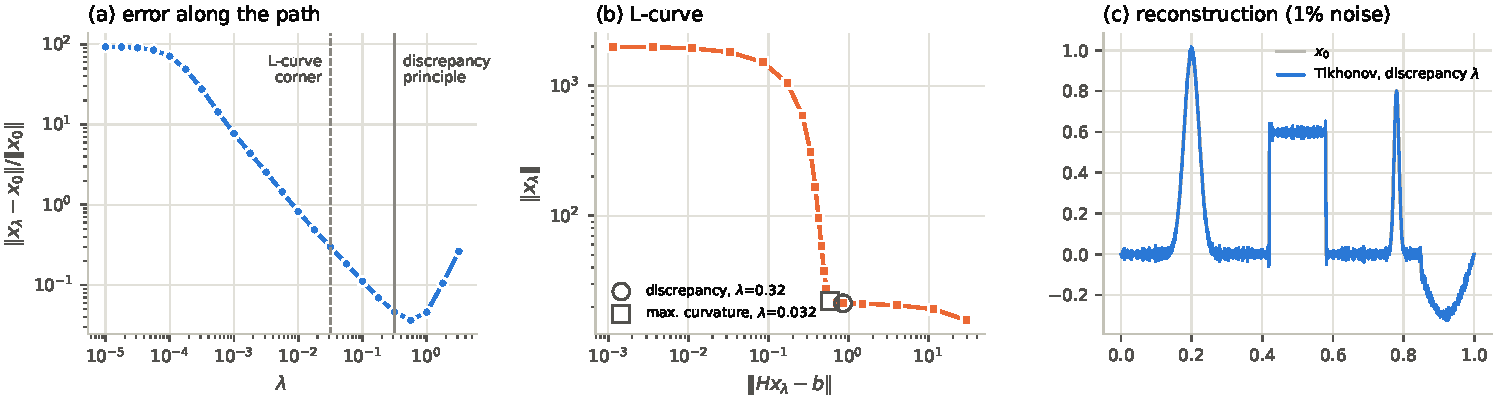
\includegraphics[width=\textwidth]{figures/m2_deblur.pdf}
\caption{Tikhonov deblurring: error along the path, L-curve (circle: discrepancy principle, square:
maximum curvature), and the discrepancy-principle reconstruction.}
\label{fig:db}
\end{figure}

\subsection{Non-Cartesian MRI with $k$-space weights}\label{subsec:mri}
\emph{Problem} (1-D model). Image $x_0$ on a centred grid of $N=2048$ pixels (piecewise constant plus a
bump). Data are $m=921$ samples of its Fourier transform at variable-density non-Cartesian
frequencies $\xi_j$, denser near $k=0$. With $x'_j=-\xi_j\bmod1$ this is exactly F5, with the
Cartesian $k$-space grid $l/N$ as the HSS column coordinates and $y=Fx$ as the unknown. A diagonal
weight on $y$ is therefore leaf-diagonal: the case this memo covers. The weight is
$L=\operatorname{diag}(1+|k_l|/k_0)$, i.e.\ the Gaussian prior with power spectrum $(1+|k|/k_0)^{-2}$
appropriate for piecewise-smooth images.

\emph{Results} (Figure~\ref{fig:mri}). Exact data: the image error is 0.120 for minimum norm and 0.098
for the weighted solution at $k_0=8$. The optimum over $k_0\in\{1,\dots,64\}$ is shallow, between 0.098
and 0.105. With 2\% noise the unweighted minimum-norm image is useless (error $2\times10^{7}$): the
variable-density nodes make $C$ severely ill-conditioned. Weighted Tikhonov at $\lambda=0.1$ restores
an error of 0.24. \emph{Tree.} Variable density is where the constructor's index-based split hurts most:
maximum HSS rank 135 with it, against 36 with the geometry-aligned tree (\texttt{mp\_tree\_aligned}).

\begin{figure}[t]
\centering
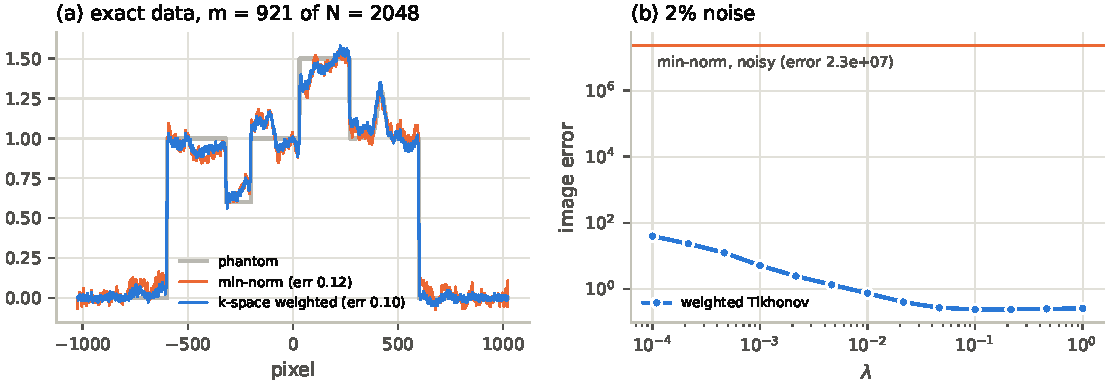
\includegraphics[width=0.85\textwidth]{figures/m2_mri.pdf}
\caption{1-D non-Cartesian MRI. (a) Exact data: minimum norm against $k$-space-weighted minimum norm.
(b) 2\% noise: weighted Tikhonov along the path against the unregularised minimum-norm image.}
\label{fig:mri}
\end{figure}

\subsection{Where the weights are not diagonal}\label{subsec:notdiag}
Two items from the list need weights that this memo does not cover (Remark~\ref{rem:nonconform}):
\begin{itemize}[leftmargin=1.4em,itemsep=1pt]
\item \emph{Seismic MWNI}: the HSS coordinates are the regular \emph{spatial} grid, but the weights live
on wavenumbers, so $L=F^*\operatorname{diag}(P^{-1/2})F$ is circulant.
\item \emph{Image-domain sparsity in MRI} (compressed sensing): the HSS coordinates are $k$-space, but the
IRLS weights live on pixels, which is again circulant.
\end{itemize}
Both are covered once $L$ is allowed to be an HSS matrix (circulants with smooth symbols are). That
needs HSS inversion and HSS products, which the repo does not have yet: the natural next step.
Alternatively, ADMM can split the weight off into its own step; then only the unweighted
minimum-norm solve is needed, in the HSS coordinates.
